\documentclass[border=2pt]{standalone}
\usepackage{pgfplots}
\pgfplotsset{compat=1.18}
\usepackage{amsmath}
\begin{document}
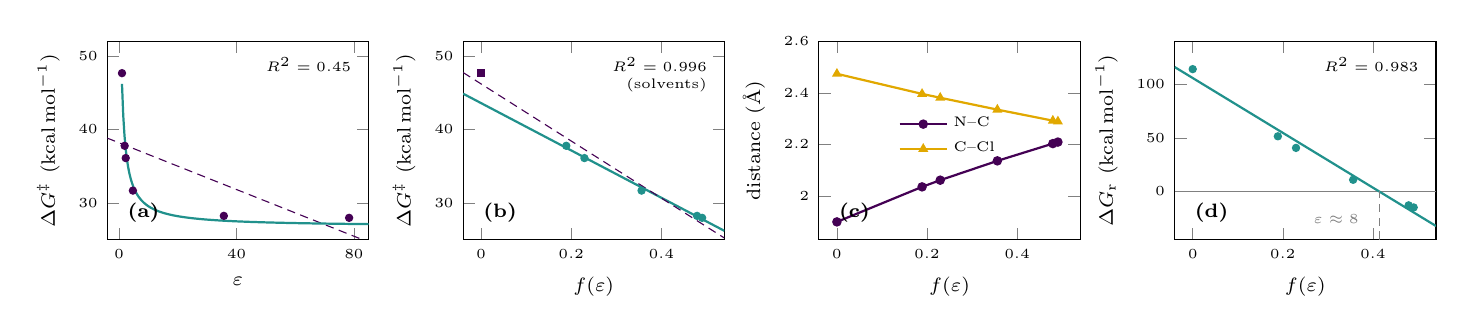
\begin{tikzpicture}
  \definecolor{c1}{HTML}{440154}
  \definecolor{c2}{HTML}{21918C}
  \definecolor{c3}{HTML}{E1A800}
  \pgfplotsset{
    every axis/.append style={
      width=4.9cm, height=4.1cm,
      tick label style={font=\tiny}, label style={font=\scriptsize},
      tick align=inside, mark size=1.3pt}}

  %--- (a) ---
  \begin{axis}[name=a,
      xlabel={$\varepsilon$}, ylabel={$\Delta G^\ddagger$ (kcal\,mol$^{-1}$)},
      xmin=-4, xmax=85, ymin=25, ymax=52, xtick={0,40,80}]
    \addplot[c1, densely dashed, domain=-4:85, forget plot] {-0.159*x + 38.188};
    \addplot[c2, thick, domain=1:85, samples=200, forget plot]
      {-38.853*(x-1)/(2*x+1) + 46.202};
    \addplot[only marks, mark=*, c1, forget plot] coordinates {
      (1.0000,47.67) (1.9113,37.78) (2.2706,36.11)
      (4.7113,31.68) (35.6880,28.24) (78.3553,27.97)};
    \node[font=\tiny, anchor=north east] at (rel axis cs:0.97,0.97) {$R^2=0.45$};
    \node[font=\scriptsize\bfseries, anchor=south west] at (rel axis cs:0.04,0.04) {(a)};
  \end{axis}

  %--- (b) ---
  \begin{axis}[name=b, at={(a.east)}, anchor=west, xshift=1.2cm,
      xlabel={$f(\varepsilon)$}, ylabel={$\Delta G^\ddagger$ (kcal\,mol$^{-1}$)},
      xmin=-0.04, xmax=0.54, ymin=25, ymax=52, xtick={0,0.2,0.4}]
    \addplot[c2, thick, domain=-0.04:0.54, forget plot] {-32.203*x + 43.589};
    \addplot[c1, densely dashed, domain=-0.04:0.54, forget plot] {-38.853*x + 46.202};
    \addplot[only marks, mark=*, c2, forget plot] coordinates {
      (0.1890,37.78) (0.2293,36.11) (0.3561,31.68) (0.4793,28.24) (0.4905,27.97)};
    \addplot[only marks, mark=square*, c1, forget plot] coordinates {(0.0000,47.67)};
    \node[font=\tiny, anchor=north east, align=right] at (rel axis cs:0.97,0.97)
      {$R^2=0.996$\\(solvents)};
    \node[font=\scriptsize\bfseries, anchor=south west] at (rel axis cs:0.04,0.04) {(b)};
  \end{axis}

  %--- (c) ---
  \begin{axis}[name=c, at={(b.east)}, anchor=west, xshift=1.2cm,
      xlabel={$f(\varepsilon)$}, ylabel={distance (\AA)},
      xmin=-0.04, xmax=0.54, ymin=1.83, ymax=2.60, xtick={0,0.2,0.4},
      legend style={font=\tiny, draw=none, fill=none,
                    at={(0.5,0.52)}, anchor=center},
      legend cell align=left]
    \addplot[c1, thick, mark=*] coordinates {
      (0.0000,1.899) (0.1890,2.035) (0.2293,2.061)
      (0.3561,2.136) (0.4793,2.203) (0.4905,2.209)};
    \addlegendentry{N--C}
    \addplot[c3, thick, mark=triangle*] coordinates {
      (0.0000,2.474) (0.1890,2.396) (0.2293,2.381)
      (0.3561,2.335) (0.4793,2.292) (0.4905,2.289)};
    \addlegendentry{C--Cl}
    \node[font=\scriptsize\bfseries, anchor=south west] at (rel axis cs:0.04,0.04) {(c)};
  \end{axis}

  %--- (d) ---
  \begin{axis}[at={(c.east)}, anchor=west, xshift=1.2cm,
      xlabel={$f(\varepsilon)$}, ylabel={$\Delta G_\mathrm{r}$ (kcal\,mol$^{-1}$)},
      xmin=-0.04, xmax=0.54, ymin=-45, ymax=140, xtick={0,0.2,0.4},
      ytick={0,50,100}]
    \addplot[gray, thin, domain=-0.04:0.54, forget plot] {0};
    \addplot[c2, thick, domain=-0.04:0.54, forget plot] {-255.7*x + 105.8};
    \addplot[only marks, mark=*, c2, forget plot] coordinates {
      (0.0000,114.09) (0.1890,51.43) (0.2293,40.59)
      (0.3561,10.85) (0.4793,-12.97) (0.4905,-14.93)};
    \addplot[gray, densely dashed, forget plot] coordinates {(0.4139,-45) (0.4139,0)};
    \node[font=\tiny, anchor=east, color=gray] at (axis cs:0.39,-26) {$\varepsilon \approx 8$};
    \node[font=\tiny, anchor=north east] at (rel axis cs:0.97,0.97) {$R^2=0.983$};
    \node[font=\scriptsize\bfseries, anchor=south west] at (rel axis cs:0.04,0.04) {(d)};
  \end{axis}
\end{tikzpicture}
\end{document}
